\chapter{Metodologia}

Este capítulo descreve a sequência de passos utilizada para extrair movimento
facial a partir de um par de imagens e transferi-lo para um modelo
tridimensional. O objetivo do sistema de animação computacional de baixo 
custo proposto é a transferência de movimento
da imagem para o modelo. Portanto a qualidade do resultado final deve ser
analisada através da comparação entre o movimento esperado e aquele efetivamente
gerado. Este trabalho não propõe uma metodologia formal para a avaliação da
qualidade final, essa avaliação é feita de forma qualitativa pela observação dos
resultados. No entanto, métricas consideradas mais quantitativas podem ser
definidas para as etapas intermediárias da aplicação e alguns experimentos são
propostos com o objetivo de avaliá-las. Este capítulo é dividido em duas partes:
a primeira descreve as etapas da aplicação proposta e a segunda descreve os
experimentos de validação dessas etapas.

\section{Etapas de Desenvolvimento}

A Figura \ref{fig:metodologia} apresenta um diagrama que ilustra as etapas da
implementação do método bem como relaciona todas as técnicas utilizadas. As
etapas apresentadas representam  o caminho dos dados dentro de cada iteração do
programa em execução.  Como sugerido pelo diagrama, as etapas são as seguintes:
Posicionamento das Câmeras para Captura das Imagens de Entrada, Rastreamento de
Pontos do Rosto, Estimação da Profundidade, Atualização dos Pesos de Mistura -
Razão de Distância, Filtros e Mistura de Poses. 

\begin{figure}
\centering
\includegraphics[width=0.9\linewidth]{figs/TG-metodologia-correta-2.png}

\caption{Diagrama completo para a animação de cada \textit{frame}. As setas
verticais representam o fluxo entre as técnicas dentro de cada iteração do
programa. As setas horizontais indicam dados provenientes de uma etapa de
calibração do sistema.}

\label{fig:metodologia}
\end{figure}



\subsection{Posicionamento das Câmeras para Captura das Imagens de Entrada}


A estrutura utilizada neste trabalho para captura de vídeo consiste na fixação
de duas \textit{webcams} comuns posicionadas paralelamente sobre uma plataforma
de madeira. Vale notar que essa é uma estrutura extremamente simples e barata para um 
sistema de animação computacional, custando em volta de cem reais. Esse é um dos fatores que 
torna o sistema proposto neste trabalho um sistema de baixo custo. A Figura 
\ref{fig:setupCameras} mostra a fixação do 
par de câmeras utilizado, sendo `$b = 18cm$'  a distância entre os centros das câmeras e 
`$a=2 cm$' a distância entre o centro de captura da câmera e a aresta do suporte.
Este parâmetro $a$ deve ser conhecido pois durante os experimentos é necessário
medir a distância do alvo ao centro das câmeras e isso é mais facilmente feito
tomando-se a distância do alvo ao suporte e utilizando o parâmetro $a$ para
recuperar a medida necessária. O parâmetro $b$ é utilizado durante a etapa de
estimação de profundidade e é equivalente ao que foi chamado de
\textit{baseline} na Figura \ref{fig:disp_cameras}. A câmera de índice 1 é
aquela que fica à direita do usuário quando este encontra-se de frente para a
montagem na Figura \ref{fig:setupCameras} e a de índice 2 é aquela que se
encontra à esquerda. Ao relacionar os pontos da câmera aos termos da Equação
\ref{eq:3d_Zequation}, chama-se o ponto alvo projetado no plano da imagem da
câmera 1 de $u$ e o ponto alvo projetado no plano da imagem da câmera 2 de $u'$.
Além disso, ao conectar as câmeras às entradas USB do computador que roda a
aplicação, deve-se conectar primeiramente a câmera 1 e em seguida a câmera 2.
Isso deve ser feito para que o programa localize corretamente as câmeras,
definindo qual imagem de entrada é proveniente da câmera da direita e qual é
proveniente da câmera da esquerda. 


\begin{figure}[!htb]
\centering
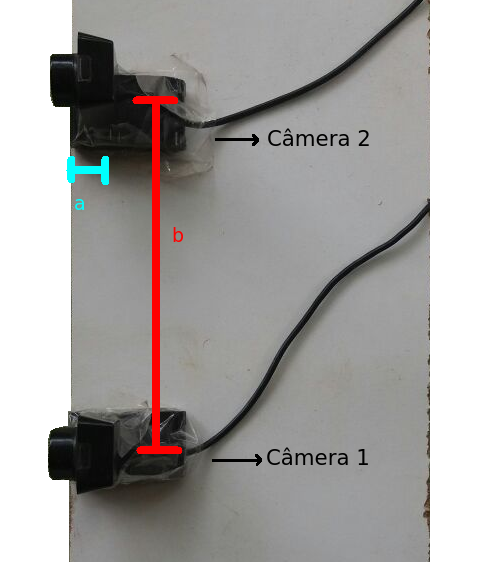
\includegraphics[width=0.7\textwidth]{figs/setupExperimento-marcado_edit-2.png}
\caption{Fixação das câmeras. Estrutura utilizada neste trabalho para a captura das imagens de entrada.}
\label{fig:setupCameras}
\end{figure}



\subsection{Rastreamento de Pontos do Rosto}

O rastreamento de pontos do rosto é a segunda etapa do processo iterativo de
animação implementado neste trabalho. Como pode ser visto na Figura
\ref{fig:metodologia}, em cada iteração do programa em execução as duas imagens
de entrada passam por esse processo separadamente.

Para fins de rastreamento de pontos do rosto, utiliza-se a
\nomenclature{SDK}{\textit{Software Development Kit}} \textit{Software
Development Kit} (SDK) \textit{CSIRO Face Analysis} \cite{cox2013csiro}
desenvolvida utilizando a biblioteca \nomenclature{OpenCV}{\textit{Open Source
Computer Vision}} \textit{Open Source Computer Vision} (OpenCV) para
representação e manipulação de imagens e vídeos. Para que ocorra o rastreamento
de pontos exige-se que a imagem de entrada esteja no formato \textit{grayscale}
(níveis de cinza). Caso não esteja, deve-se primeiramente transformar a imagem
de entrada para este formato. 

Para rastrear pontos da face a SDK implementa a técnica RMLS introduzida na
fundamentação. O Algoritmo \ref{alg:rlms} descreve de forma simplificada os
passos tomados para se obter o rastreamento \cite{saragih2011deformable}. A
variável $\mathbf{p}$ no algoritmo representa os parâmetros do PDM e com ela
calculada pode-se obter a posição dos pontos de interesse através da Equação
\ref{eq:PDM-equation}. Um detalhamento da técnica pode ser encontrado em
\cite{saragih2011deformable}.

\begin{algorithm}[!htb]
\caption{RLMS (\textit{Regularized landmark mean-shift})}\label{alg:rlms}
\begin{algorithmic}[1]
\Require{$\mathcal{I}$ e $\mathbf{p}$} \Comment{$\mathcal{I}$ sendo a imagem e $\textbf{p}$ como definido na Equação \ref{eq:alg1}}
\State Computar respostas [Equações \ref{eq:alg1}]
   \While{nao{\_}convergiu(\textbf{p})}
   \State Linearizar o modelo de forma [Equação \ref{eq:alg2}]
   \State Computar os vetores do deslocamento da média [Equação \ref{eq:alg3}]
   \State Computar a atualização dos parâmetros PDM [Equação \ref{eq:alg4}]
   \State Atualizar parâmetros: $\textbf{p} \leftarrow \textbf{p} + \Delta\textbf{p}$
   \EndWhile
   \State \textbf{return} $\textbf{p}$
\end{algorithmic}
\end{algorithm}





O resultado do rastreamento é um arranjo de 66 pontos contendo os valores das
coordenadas $(x,y)$ na imagem de cada ponto chave. A SDK ordena os pontos
retornados de forma que cada ponto chave esteja sempre em uma mesma posição do
arranjo. Os pontos rastreados e a numeração associada a cada um deles são
mostrados na  Figura \ref{fig:tracked-facial-points}. 

\begin{figure*}
\centering
\begin{tabular}{cc}
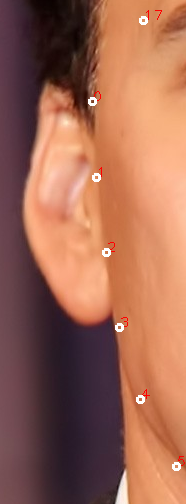
\includegraphics[width=0.4\linewidth, height=5cm]{figs/nick-marked-l-ear.png} &
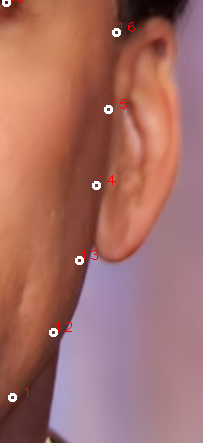
\includegraphics[width=0.4\linewidth, height=5cm]{figs/nick-marked-r-ear.png} \\
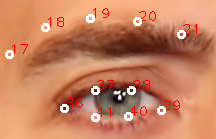
\includegraphics[width=0.4\linewidth, height=5cm]{figs/nick-marked-l-eye.png} &
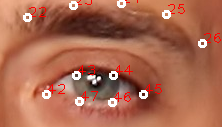
\includegraphics[width=0.4\linewidth, height=5cm]{figs/nick-marked-r-eye.png} \\
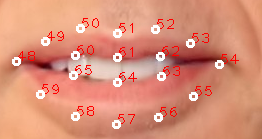
\includegraphics[width=0.4\linewidth, height=5cm]{figs/nick-marked-mouth.png} &
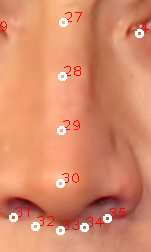
\includegraphics[width=0.4\linewidth, height=5cm]{figs/nick-marked-nose.png} \\
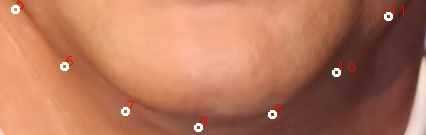
\includegraphics[width=0.4\linewidth, height=5cm]{figs/nick-marked-queixo.png} &
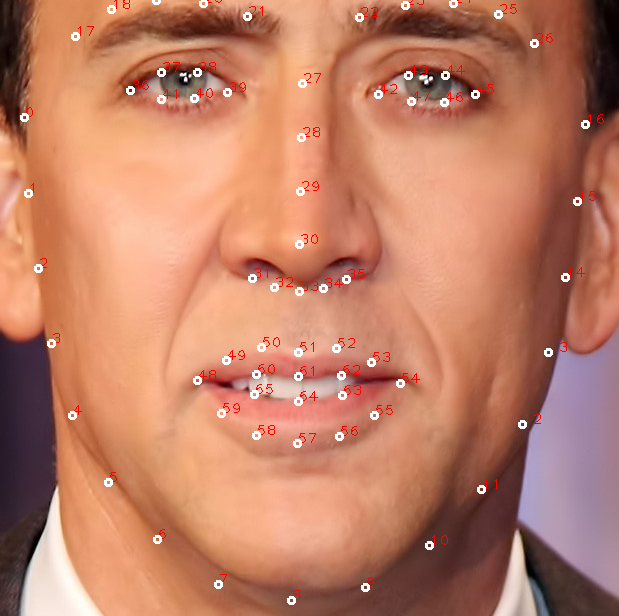
\includegraphics[width=0.4\linewidth, height=5cm]{figs/nick-marked.png}
\end{tabular}
\caption{Pontos retornados pelo rastreamento facial e a numeração associada a cada ponto. A imagem sobre a qual se realiza o rastreamento (retirado de \cite{nicolas}).}
\label{fig:tracked-facial-points}
\end{figure*}


Além dos pontos retornados, um valor entre zero e dez representando a qualidade
da detecção é fornecido ao final de cada rastreamento. Esse valor serve para
avaliar se a detecção do quadro atual deve ser utilizada, para assim atualizar a
malha tridimensional: caso o valor da qualidade de detecção seja zero em uma
iteração, o modelo não é atualizado. Além disso, uma qualidade de zero indica
que o rastreamento perdeu completamente os pontos de interesse e é necessário
reinicializar o rastreador para que a detecção tenha chance de ser realizada com
sucesso na próxima iteração.

Além disso, como o rastreamento é aplicado independentemente a cada uma das
imagens de entrada, é importante que se mantenham dois rastreadores
inicializados e atualizados independentemente. Isso deve ser feito pois a SDK
reutiliza informações de estados anteriores para acelerar o rastreamento no
quadro atual e não se deve misturar o estado do rastreamento na imagem esquerda
com o estado do rastreamento na imagem direita. 

A saída desta etapa como um todo consiste de dois conjuntos de 66 pontos
bidimensionais enumerados, uma para cada imagem, bem como dois parâmetros que
representam a qualidade do rastreamento feito em cada imagem. 

\subsection{Estimação da Profundidade}

Como ficará colocado em mais detalhes nas próxima seções, esta aplicação utiliza
a distância entre pontos do rosto para interpretar a posição que deve ser
transferida para o modelo. Sem a estimação de profundidade, a distância entre
dois pontos do rosto diminuiria a medida que o usuário se afastasse do par de
câmeras e colocaria sobre o usuário a responsabilidade de realizar gravações
sempre a uma mesma distância. Além disso, uma leve movimentação despercebida
durante as gravações poderia ser erroneamente interpretada pelo programa, já que
decisões são tomadas a partir do movimento entre os pontos e um afastamento do
usuário causaria uma redução em todas as distâncias.  A estimação da
profundidade permite que medidas retiradas da imagem sejam independentes da
distância em que o usuário se encontra das câmeras, o que garante maior
flexibilidade de uso e uma maior estabilidade na animação. Com a estimação da
profundidade é possível aproximar os valores $X$, $Y$ e $Z$ dos pontos de
interesse no sistema de coordenadas do mundo. Por exemplo, a distância entre os
dois olhos do usuário deve ser sempre a mesma e pode ser medida em centímetros e
não mais em pixeis.

A estimação da profundidade é feita utilizando-se os dois conjuntos de pontos
fornecidos pela etapa de rastreamento. Um exemplo de um par de imagens de
entrada onde o rastreamento foi aplicado e os pontos marcados pode ser observado
na Figura \ref{fig:input_images}. As imagens tiradas em uma mesma iteração do
programa por câmeras diferentes mostram o usuário em  uma posição ligeiramente
deslocada em relação a outra, e é justamente essa diferença horizontal que é
utilizada para estimar a profundidade. Além disso, uma vez estimada a
profundidade, pode-se corrigir a posição horizontal dos pontos de
interesse\footnote{Vale lembrar que assume-se que os centros de captura das
câmeras estão alinhados verticalmente e, portanto, não espera-se diferença entre
as coordenadas Y de um mesmo ponto do rosto nas duas imagens.}.

\begin{figure}[!htb]
  \centering
  \begin{subfigure}[]{\label{fig:filter3}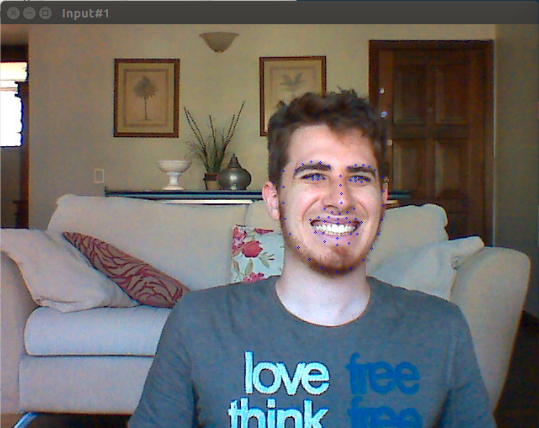
\includegraphics[width=0.45\textwidth]{./figs/TG_input_image1.png}}
  \end{subfigure}   
  \begin{subfigure}[]{\label{fig:filter4}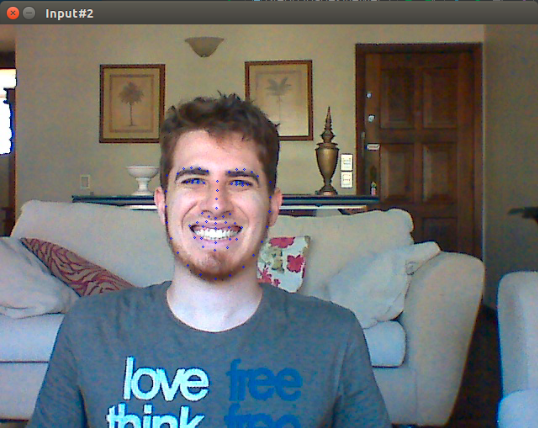
\includegraphics[width=0.45\textwidth]{./figs/TG_input_image2.png}}
  \end{subfigure}

  \caption{ Imagens extraídas da câmera 1 (a) e da câmera 2 (b) em uma mesma
  iteração do programa em execução. Ao comparar as duas imagens, nota-se que o
usuário aparece deslocado horizontalmente em uma imagem quando comparado a
outra. Os pontos de interesse foram rastreados e marcados com círculos azuis.}

\label{fig:input_images}
\end{figure}

Como o cojunto de pontos rastreados é sempre ordenado da mesma maneira, é fácil
localizar o mesmo ponto do rosto em cada uma das imagens: basta tomar os mesmos
índices em cada um dos vetores retornados pela etapa de rastreamento. Esse
mapeamento de pontos é utilizado para estimar a posição no mundo de cada um dos
pontos rastreados, isso é feito através de uma semelhança de triângulos, como
foi resumido na Equação \ref{eq:3d_Zequation} apresentada na fundamentação
teórica.

Vale notar que para a aplicação da Equação \ref{eq:3d_Zequation} deve-se
anteriormente conhecer a distância focal de cada uma das câmeras, o que pode ser
obtido pela utilização da ferramenta \textit{Calibration Toolbox}, uma extensão
disponível para Matlab. O processo de calibração de uma câmera por meio dessa
ferramenta consiste na captura de vinte imagens de um tabuleiro de xadrez em
diferentes posições. Após a marcação manual das extremidades desse tabuleiro, o
algoritmo de calibração realiza um processo de detecção em cada uma das imagens
de um conjunto de pontos conhecidos - as quinas de cada um dos quadrados do
tabuleiro de xadrez . O mapeamento desses pontos em cada uma das imagens em
conjunto com o conhecimento do tamanho real de cada uma das casas do tabuleiro
permite determinar a matriz de calibração da câmera, que inclui, dentre outros
valores, os parâmetros intrínsecos da câmera. Um exemplo do conjunto de imagens
utilizado durante a etapa de calibração pode ser observado na Figura
\ref{fig:calib_imagens}.  A calibração\footnote{O termo `calibração' aqui
significa a realização de um processo que estima os parâmetros de interesse.
Nenhuma modificação é aplicada sobre os sensores em si.} é feita após o processo
de fixação das câmeras e os resultados guardados para utilização enquanto os
resultados da estimação de profundidade se mostrarem satisfatórios. Vale notar
que choques ocasionais aplicados a montagem podem alterar os parâmetros das
câmeras e requerer uma recalibração destes. 

\begin{figure}[h!]
\centering
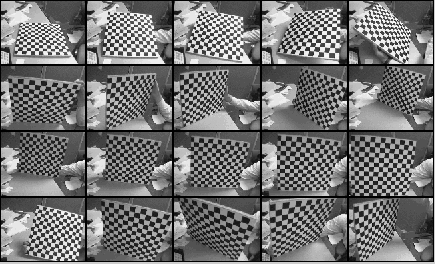
\includegraphics[width=.6\linewidth]{figs/TG_calib_images.png}
\caption{Exemplo de imagens utilizadas em uma calibração (retirado de \cite{bouguetML}).}
\label{fig:calib_imagens}
\end{figure}

A matriz $KK$ dos parâmetros intrínsecos da câmera obtida por uma calibração
feita utilizando a \textit{Calibration Toolbox for Matlab} é mostrada na Equação
\ref{eq:calib_matIntrinseca}.

\begin{align}
KK =
\left[\begin{array}{ccc}
f_c(1) & alpha_c*f_c(1) & cc(1)\\
0 & f_c(2) & cc(2)\\
0 & 0 & 1
\end{array}\right]
\label{eq:calib_matIntrinseca}
\end{align}

Onde $f_c(1)$ e $f_c(2)$ são as distâncias focais descritas em unidades de
pixeis horizontais e verticais, o coeficiente $alpha_c$ é o ângulo entre os
eixos de coordenadas $x$ e $y$ e os valores de $cc(1)$ e $cc(2)$ representam as
coordenadas $x$ e $y$ do ponto principal da câmera.

Caso seja considerado um pixel quadrado, ou seja, $alpha_c = 0$ e $f_c(1) =
f_c(2)$, essa matriz intrínseca será igual a matriz definida na Equação
\ref{eq:3d_matIntrinseca}.

De posse de todas as variáveis é então possível estimar o valor $Z$ de um ponto
no mundo e com isso estimar também os valores $X$ e $Y$ deste mesmo ponto. O
cálculo dos valores $X$ e $Y$ é feito por meio das Equações \ref{eq:3d_realX1} e
\ref{eq:3d_realX2} e das Equações \ref{eq:3d_realY1} e \ref{eq:3d_realY2},
respectivamente.    

Sumarizando, a etapa de estimação de profundidade utiliza os \textbf{dois}
conjuntos de pontos \textbf{bidimensionais} provenientes da etapa de
rastreamento para produzir \textbf{um} conjunto de sessenta e seis pontos
\textbf{tridimensionais} contendo cada um os valores $(X,Y,Z)$ referentes às
coordenadas de cada ponto rastreado no sistema de coordenadas do mundo. Além de
adicionar a componente de profundidade, esta etapa retorna os valores em
centímetros das componentes dos elementos do conjunto produzido.

\subsection{Atualização dos Pesos de Mistura - Razão de Distância}

Até este ponto a aplicação obteve uma estimação para as coordenadas espaciais de
um conjunto de pontos de interesse da face humana. Passa-se agora para a etapa
de extração de informação de pose a partir desse conjunto de pontos. Como será
detalhado na próxima seção, isso é feito por meio da técnica de mistura de poses
que requer como entrada um vetor de pesos. O objetivo desta etapa pode ser posto
como inferir um vetor de pesos que adequadamente produzirá uma mistura de poses
cujo resultado se assemelha com a expressão facial na imagem de entrada.

Define-se cada uma das componentes do vetor de peso independentemente como uma
\textbf{razão de distâncias} entre dois pontos do conjunto de pontos fornecidos
pela etapa de rastreamento. A razão é tomada entre a distância entre os pontos
medida no quadro considerado e a distância entre esses mesmos pontos em quadros
de uma etapa de calibração. Como o interesse é a variação percentual, o que é
medido é de fato a fração que a distância atual se encontra entre a distância
máxima e a mínima medida para o par de pontos.

Seja o peso $w_i^j$ associado com o par de pontos $(\bm{p_1^i}, \bm{p_2^i})$ no
quadro j e seja $d_i^j = |\bm{p_1^i} - \bm{p_2^i}|$ a distância medida entre
esse par de pontos nesse quadro, o peso da i-ésima pose é dado por:

\begin{equation}
	w_i^j = \frac{|d_i^j - d_i^{\text{min}}|}{|d_i^{\text{max}} - d_i^{\text{min}}|}
   \label{eq:pesos1}
\end{equation}

onde $d_i^{\text{min}}$ e $d_i^{\text{max}}$ são as distâncias mínimas e máximas
respectivamente para o par de pontos associado ao peso $w_i$ obtidas em uma
etapa de calibração. 

A Equação \ref{eq:pesos1} descreve poses onde um aumento na razão de distância
significa um aumento no peso da pose associada. No caso de poses onde o oposto
deve acontecer, ou seja, uma diminuição da razão de distância significa um
aumento do peso da pose associada, a equação de peso é dada por: 

\begin{equation}
	w_i^j = 1 - \frac{|d_i^j - d_i^{\text{min}}|}{|d_i^{\text{max}} - d_i^{\text{min}}|}
    \label{eq:pesos2}
\end{equation}

A Equação \ref{eq:pesos2} é utilizada, por exemplo, para o peso associado a pose
que fecha um dos olhos. Nesta pose, quanto maior o peso associado, mais fechado
o olho se encontra. Por outro lado, quando mais fechado o olho, menor a
distância vertical entre pontos ao longo das pálpebras de cima e de baixo desse
olho.

Nota-se que as equações apresentadas descrevem cada peso como um valor entre 0 e
1. No entanto, o modelo de poses utilizado requer que a soma dos pesos resulte
em 1. Para garantir essa condição, o peso da pose neutra é escolhido como:

\begin{equation}
	w_{\text{neutra}}^j = 1 - \sum_{i} w_i^j
    \label{eq:pesos3}
\end{equation}

onde i varia no intervalo de índices das poses de ação (as poses excluindo a
pose neutra).

Resumindo, para cada pose disponível na mistura de poses escolhe-se dois pontos
do conjunto de pontos da etapa de estimação de profundidade e define-se o peso
da pose associada a partir da comparação entre a  distância entre esses dois
pontos no quadro atual e a a distância entre esses dois pontos em quadros de uma
etapa de calibração. Os quadros da etapa de calibração são dois: um
correspondente a 0\% da pose e outro correspondendo a 100\% da aplicação da
pose.

O par de pontos utilizados para cada uma das poses disponíveis para mistura são
listados na Tabela \ref{tab:sensors}. Para cada ponto apresenta-se o índice
correspondente no vetor de 66 pontos da etapa de rastreamento, bem como uma
descrição de sua localização no rosto. O mapeamento entre o índice de pose e a
sua descrição é apresentado na Tabela \ref{tab:poses-descr}. 

\begin{table}[!htb]
\centering
\begin{tabular}{|l|l|l|l|l|}
\hline
k &  $i_k$ & descrição de $p_{i_k}$ & $j_k$ & descrição de $p_{j_k}$ \\ \hline
1 &  54 & canto esquerdo da boca & 48  & canto direito da boca \\ \hline
2 & 24 & centro da sobrancelha esquerda & 42 & canto direito do olho esquerdo \\ \hline
3 & 19 & centro da sobrancelha direita & 39 & canto esquerdo do olho direito \\ 	\hline
4 &  43 & canto superior do olho esquerdo & 47 & canto inferior do olho esquerdo \\ \hline
5 &  37 & canto superior do olho direito & 41 & canto inferior do olho direito \\ \hline
6 &  61 & centro inferior do lábio superior& 64 & centro superior do lábio inferior \\ \hline
\end{tabular}
\caption{Pares de pontos utilizados para razão de distâncias. O peso $w_k$ está associado com o par $(p_{i_k},p_{j_k})$. Os índices dos pontos podem ser comparados com os índices da Figura \ref{fig:tracked-facial-points}}
\label{tab:sensors}
\end{table}

\begin{table}[!htb]
\centering
\begin{tabular}{|l|l|}
\hline
k & pose k  \\ \hline
1 & sorrir  \\ \hline
2 & levantar da sobrancelha esquerda\\ \hline
3 & levantar da sobrancelha direita \\ 	\hline
4 & fechar do olho esquerdo  \\ \hline
5 & fechar do olho direito \\ \hline
6 & abrir da boca  \\ \hline
\end{tabular}
\caption{Mapeamento do índice da pose no vetor de pesos com ação realizada pela aplicação da pose.}
\label{tab:poses-descr}
\end{table}



\subsection{Filtros}

Os pesos de mistura calculados anteriormente não são utilizados diretamente no
processo de mistura de poses, antes disso eles são filtrados. O objetivo dos
filtros digitais é remover componentes de altas frequências associadas a ruídos
presentes no processo de captura de imagem e na própria detecção. 

Os filtros digitais projetados para suavizar a detecção foram filtros FIR
passa-baixas, implementados no domínio do tempo por meio de equações de
diferenças. Para a implementação dos filtros é necessário que se mantenha em
memória os valores das entradas em instantes de tempo anteriores. Uma primeira
implementação consiste em mover cada uma das entradas para a próxima posição do
vetor de entradas anteriores em cada atualização do filtro. Para evitar esse
laço de deslocamento, utiliza-se nesta aplicação a técnica de \text{buffer}
circular que mantém um índice para a posição mais recente e atualiza esse índice
ao invés de atualizar a posição dos dados em si.


Para o projeto dos coeficientes do filtro, duas técnicas foram utilizadas:
filtros de média móvel e projeto por janela. Para este último, a janela de
Hamming foi utilizada para realizar cortes sobre o filtro de resposta infinita
que geraria a resposta ideal. O motivo de se projetar vários filtros é permitir
que diferentes bandas sejam filtradas em cada um dos pesos de mistura. Isso se
faz necessário pois, por exemplo, enquanto altas frequências representam ruídos
na detecção da ação de sorrir, elas podem ser necessárias para capturar
movimentos rápidos como o piscar de olhos. Durante a execução do programa,
cursores de seleção permitem selecionar o filtro utilizado para cada um dos
pesos de mistura.

Os gráficos na Figura \ref{fig:filter-design-frequency-response} mostram a
resposta em frequência de cada filtro. O Filtro de Média Móvel de Hamming é
descrito na Equação \ref{eq:filter-hanning}.

\begin{align}
\label{eq:filter-hanning}
y(n) = \frac{1}{4}(1 x(n) + 2 x(n-1) + x(n-2))
\end{align}

Os filtros projetados com a técnica da janela seguem a seguinte equação:

\begin{equation}
	y(n) = \sum_{k=0}^L b_k x(n-k)
\end{equation}

Para L=16, a Tabela \ref{tab:fir-filters-coefs} mostra os coeficientes para
alguns dos filtros projetados pela técnica de corte com janela de Hanning.

\begin{table}
\centering
\begin{tabular}{|l|l|l|l|}\hline
k \/$w_c$ & $0.1\pi$ & $0.1\pi$ & $0.1\pi$ \\ \hline
  0	& 0,0025	&   -0,0000	&		0,0030 \\		
 1	& 0,0057	&   -0,0052	&	   -0,0050 \\	
 2	& 0,0147	&    0,0000	&	    0,0067 \\	
 3	& 0,0315	&    0,0232	&	   -0,0000 \\	
 4	& 0,0555	&   -0,0000	&	   -0,0252 \\	
 5	& 0,0834	&   -0,0761	&	    0,0721 \\	
 6	& 0,1099	&    0,0000	&	   -0,1306 \\	
 7	& 0,1289	&    0,3077	&	    0,1801 \\	
 8	& 0,1358	&    0,5009	&	    0,7979 \\	
 9	& 0,1289	&    0,3077	&	    0,1801 \\	
10	& 0,1099	&    0,0000	&	   -0,1306 \\	
11	& 0,0834	&   -0,0761	&	    0,0721 \\	
12	& 0,0555	&   -0,0000	&	   -0,0252 \\	
13	& 0,0315	&    0,0232	&	   -0,0000 \\	
14	& 0,0147	&    0,0000	&	    0,0067 \\	
15	& 0,0057	&   -0,0052	&	   -0,0050 \\	
16	& 0,0025	&   -0,0000	&	    0,0030 \\
\hline
\end{tabular}

\caption{Coeficientes para os filtros projetados com técnica de janela,
utilizando a janela de Hanning.}

\label{tab:fir-filters-coefs}
\end{table}


\begin{figure}[!hbt]
\centering
\begin{tabular}{cc}
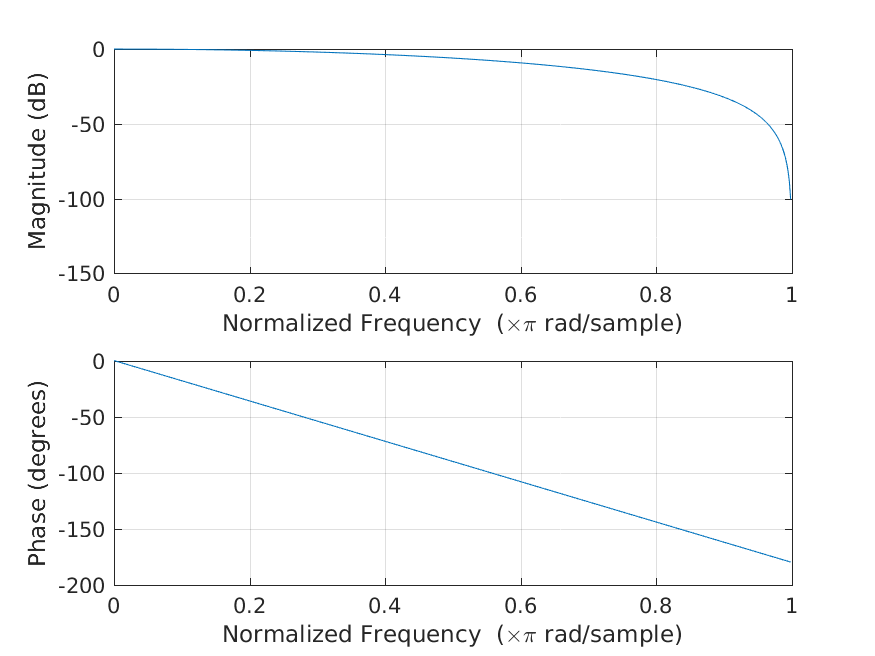
\includegraphics[width=0.45\linewidth]{figs/filter-response-hanningFilter.png} &
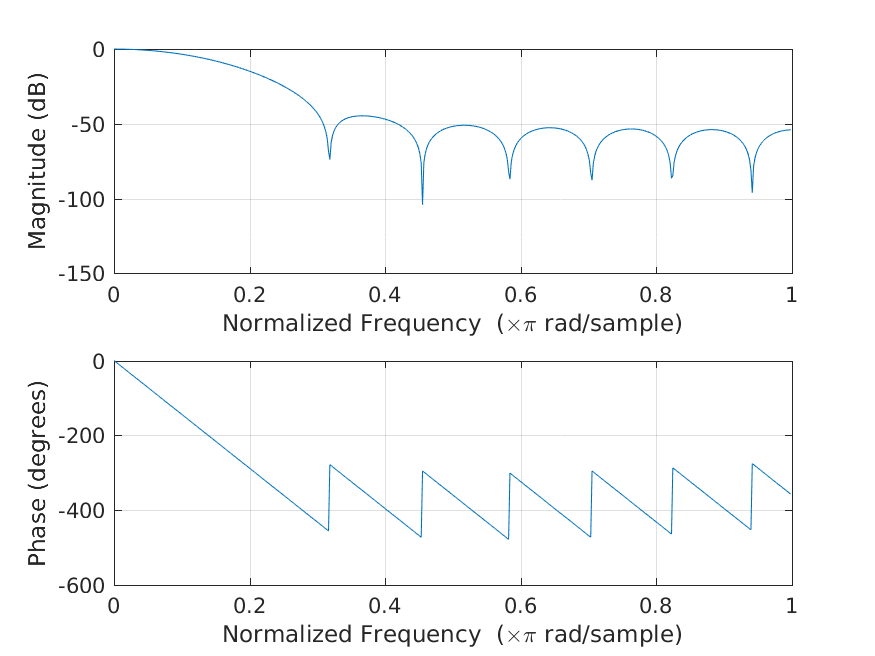
\includegraphics[width=0.45\linewidth]{figs/filter-response-wc_0_1pi.png}\\
(a) Filtro de Média móvel de Hamming & (b) Projeto com janela de Hanning $w_c=\frac{\pi}{10}$ \\
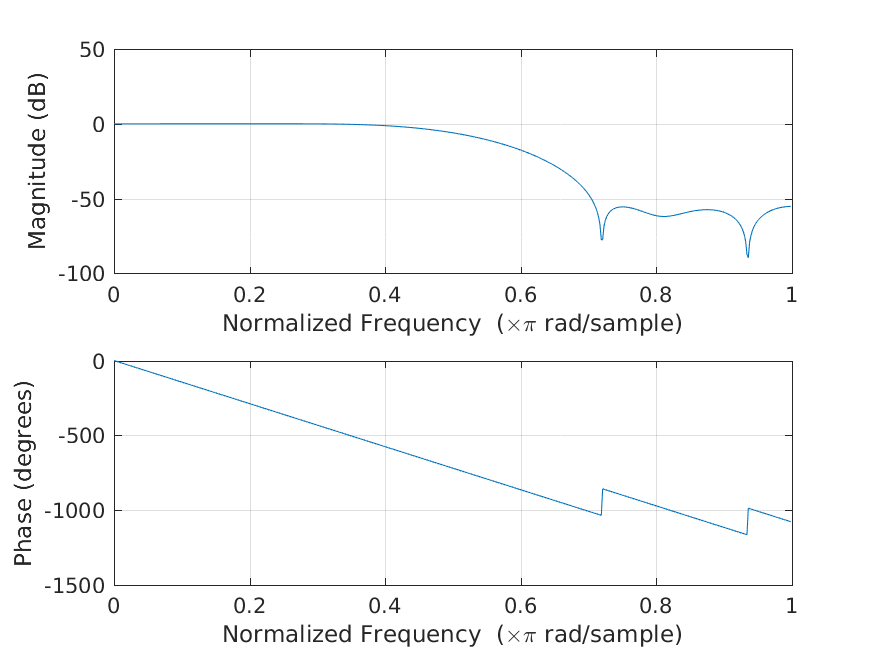
\includegraphics[width=0.45\linewidth]{figs/filter-response-wc_0_5pi.png} &
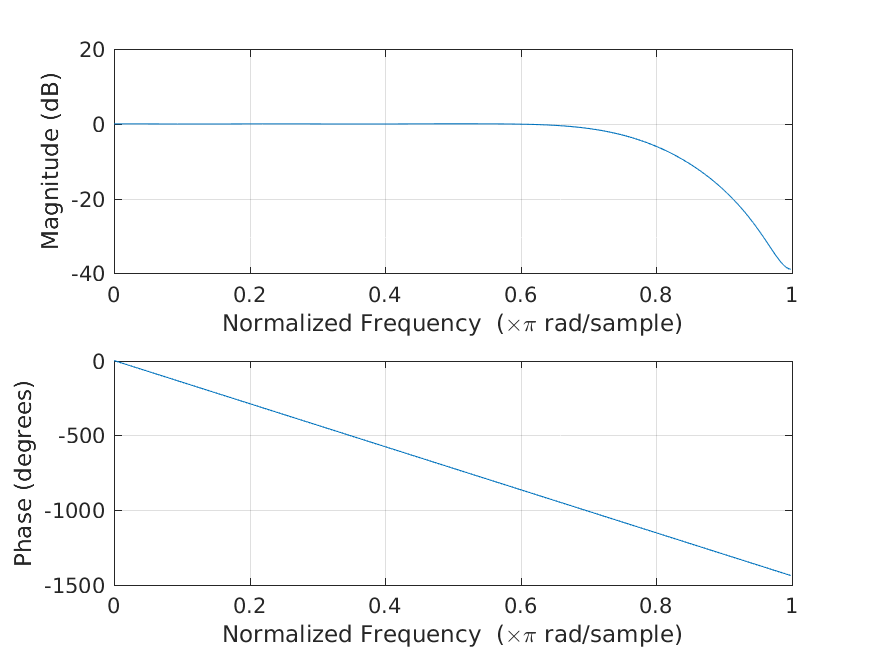
\includegraphics[width=0.45\linewidth]{figs/filter-response-wc_0_8pi.png} \\
(c) Projeto com janela de Hanning $w_c=\frac{\pi}{2}$ & (d) Projeto com janela de Hanning $w_c=\frac{4\pi}{5}$ \\
\end{tabular}

\caption{Magnitude e fase da resposta em frequência para alguns dos filtros
utilizados na aplicação.}

\label{fig:filter-design-frequency-response}
\end{figure}

\subsection{Mistura de Poses}

O conceito básico por trás da Mistura de Poses está em criar poses
intermediárias a partir da interpolação linear de poses pré-definidas.

A pose base utilizada para a mistura de poses deve ser uma onde todas as razões
de distância estão no mínimo, ou seja, deve ser uma pose onde a face esteja em
repouso. O modelo utilizado para a pose neutra é mostrada na Figura
\ref{fig:blend-shapes-base-model}.

\begin{figure*}[!htb]
   \centering
  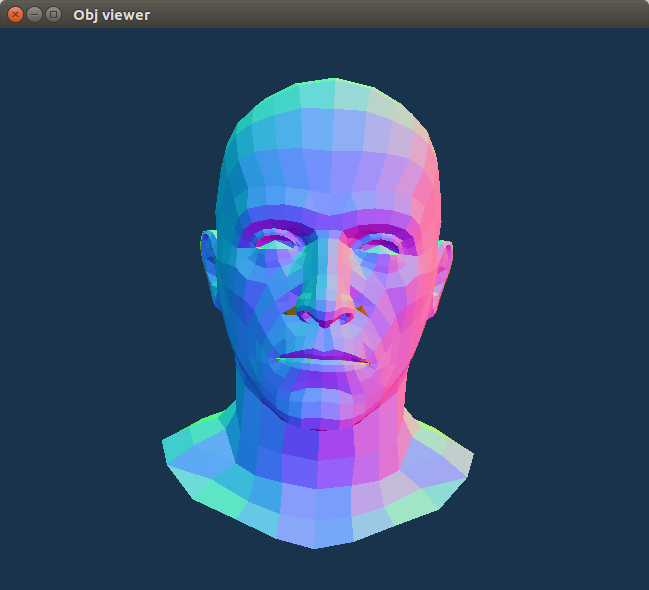
\includegraphics[width=0.8\linewidth]{./figs/rosto-neutro.png}
\caption{Pose base (neutra).}
\label{fig:blend-shapes-base-model}
\end{figure*}

Aos demais modelos renderizados é atribuído um peso de mistura definido como a
saída de um filtro que recebe como entrada uma sequência de valores de uma razão
de distância.

Alguns detalhes são necessários para que a mistura de poses ocorra com sucesso.
Dentre eles, é necessário que os pontos na malha do modelo apareçam enumerados
na mesma ordem em todas as poses utilizadas para a mistura. Isso pode ser
garantido requerendo-se do software que exporta os modelos para formato de
arquivo OBJ que mantenha os pontos na mesma ordem. Essa é uma opção comum nos
softwares de modelagem, mas que nem sempre é habilitada por padrão e o requisito
de manutenção da ordem dos pontos deve ser informado ao artista responsável pela
produção dos modelos para que ele configure o software adequadamente. Outro
requisito é que os modelos utilizem um mesmo sistema de coordenas e que os
triângulos da malha utilizem uma mesma indexação de VBOs. O primeiro requisito
não apresentou problemas na realização deste trabalho, sendo suficiente centrar
o objeto em (0,0,0), porém o segundo requisito apresentou problemas. Enquanto o
número e a ordem na listagem de triângulos se mantém o mesmo, verificou-se que
os softwares de modelagem nem sempre mantêm a mesma ordem da listagem dos pontos
de um dado triângulo. Ou seja, os pontos de um triângulo são sempre os mesmos em
dois arquivos OBJ, mas não necessariamente aparecem listados na mesma ordem, o
que causa problemas durante o processo de mistura. Para resolver este problema,
a construção da malha por meio de triângulos para todos os modelos utilizados é
feita com a listagem de triângulos da malha da pose neutra. Ou seja, os
triângulos são definidos pela pose neutra e carrega-se dos OBJ de cada uma das
outras poses apenas o posicionamento dos pontos da malha.

Caso os arquivos sejam carregados adequadamente e a mistura de poses seja
realizada com sucesso é possível verificar uma transição natural entre o modelo
da Pose Neutra para qualquer outro modelo pré-definido ao fazer a mistura de
poses utilizando-se somente a pose neutra e uma das outras poses.

Como o modelo final renderizado é uma interpolação dos pontos de todos os
modelos após a aplicação dos pesos calculados, esse modelo será igual a uma pose
pré-definida apenas se a razão de distância referente a ela for máxima, enquanto
todas as outras forem mínimas. Caso contrário, se o rosto não está em repouso, o
modelo final sempre será igual a uma pose intermediária. As poses pré-definidas
utilizadas neste trabalho são mostradas na Figura
\ref{fig:blend-shapes-base-simple-shapes1} e na Figura
\ref{fig:blend-shapes-base-simple-shapes2}.



\begin{figure}[!htpb]
  \centering
  \begin{subfigure}[Pose Olho Esquerdo]{\label{fig:pose_l_eye}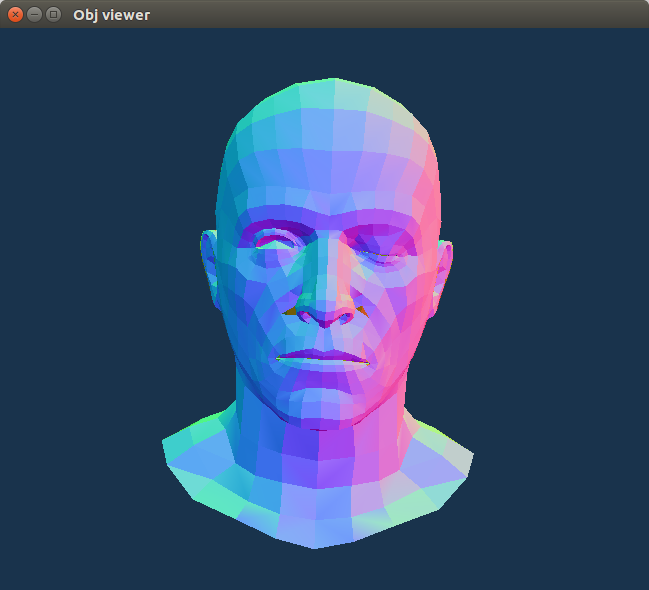
\includegraphics[width=0.4\textwidth]{./figs/left-closed-eye.png}}
  \end{subfigure}   
  \begin{subfigure}[Pose Olho Direito]{\label{fig:pose_r_eye}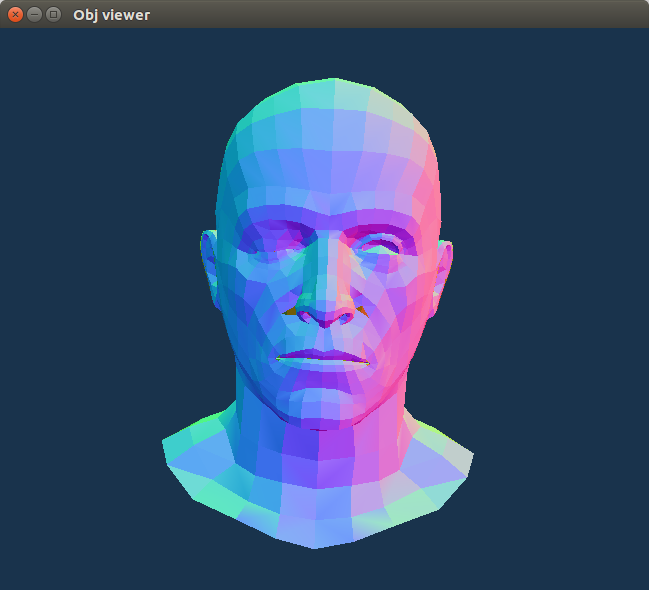
\includegraphics[width=0.4\textwidth]{./figs/right-closed-eye.png}}
  \end{subfigure}
  
  \begin{subfigure}[Pose Sobrancelha Esquerda]{  \label{fig:pose_l_eyebrow}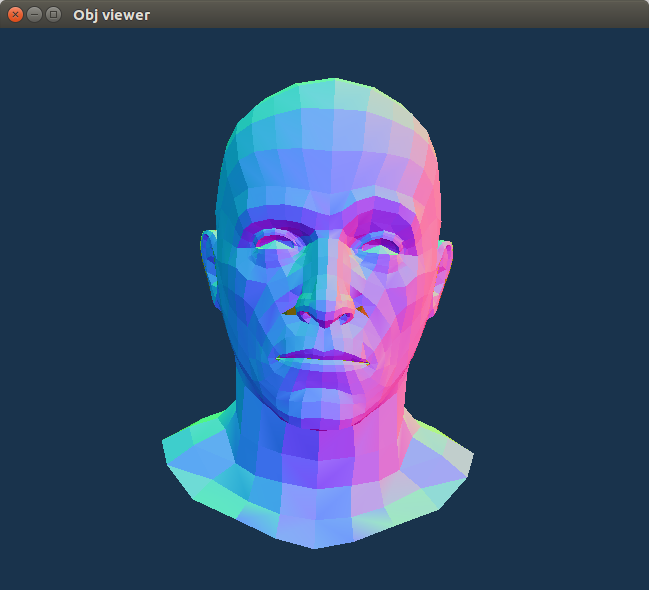
\includegraphics[width=0.4\textwidth]{./figs/left-eyebrow.png}}
  \end{subfigure} 
  \begin{subfigure}[Pose Sobrancelha Direita]{  \label{fig:pose_r_eyebrow}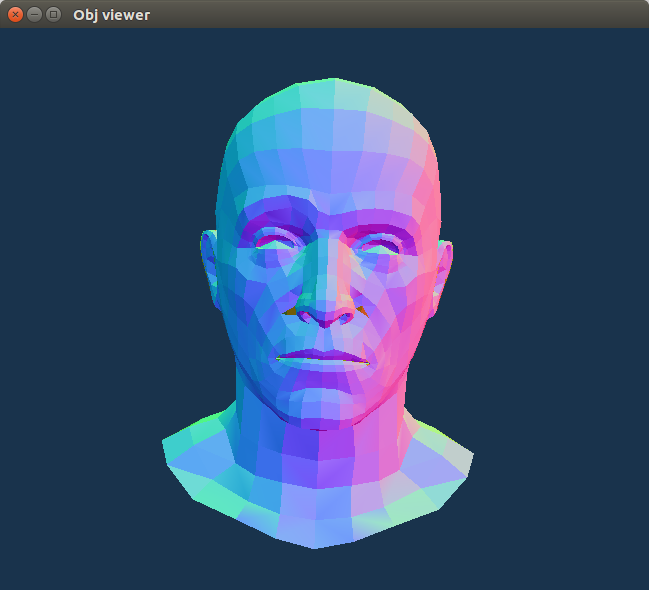
\includegraphics[width=0.4\textwidth]{./figs/right-eyebrow.png}}
  \end{subfigure}
  
  \begin{subfigure}[Pose Boca Fechada]{\label{fig:pose_c_mouth}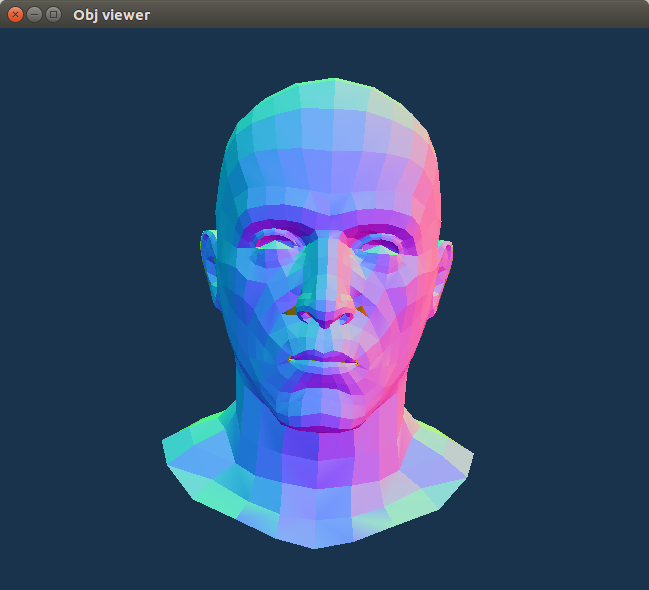
\includegraphics[width=0.4\textwidth]{./figs/mouth-closed.png}}
  \end{subfigure}
  \begin{subfigure}[Pose Boca Aberta]{\label{fig:pose_o_mouth}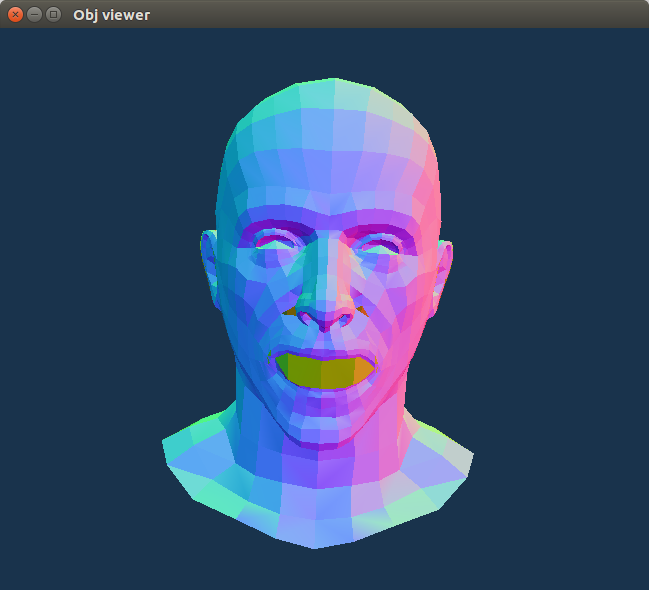
\includegraphics[width=0.4\textwidth]{./figs/open-mouth.png}}
  \end{subfigure}

  \caption{Exemplos de modelos usados como poses pré-definidas.}

  \label{fig:blend-shapes-base-simple-shapes1}
\end{figure}



\begin{figure}[!htpb]
  \centering
  \begin{subfigure}[Pose Bochecha Esquerda]{\label{fig:pose_l_cheek}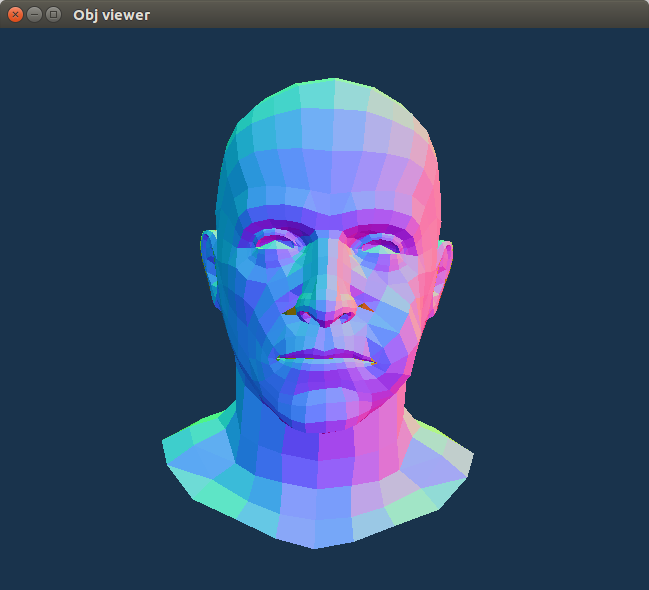
\includegraphics[width=0.4\textwidth]{./figs/bochecha-esquerda.png}}
  \end{subfigure}   
  \begin{subfigure}[Pose Bochecha Direita]{\label{fig:pose_r_cheek}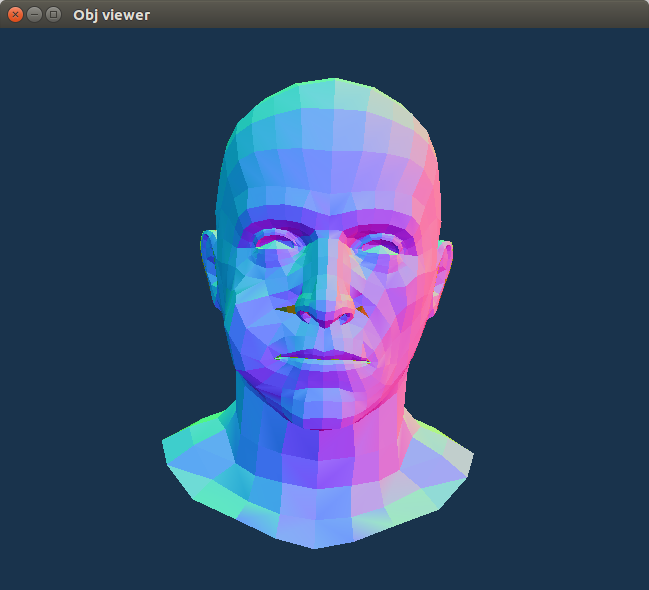
\includegraphics[width=0.4\textwidth]{./figs/bochecha-direita.png}}
  \end{subfigure}
  
  \begin{subfigure}[Pose Sorrindo]{  \label{fig:pose_happy}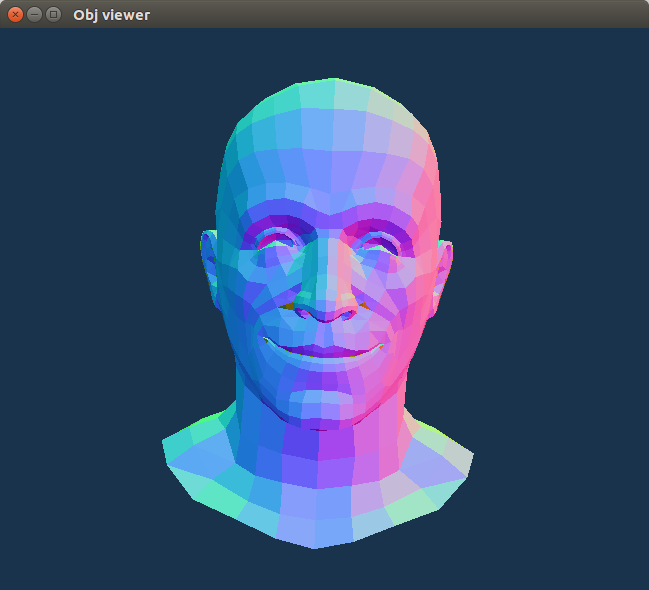
\includegraphics[width=0.4\textwidth]{./figs/rosto-feliz.png}}
  \end{subfigure} 
  \begin{subfigure}[Pose Bravo]{  \label{fig:pose_angry}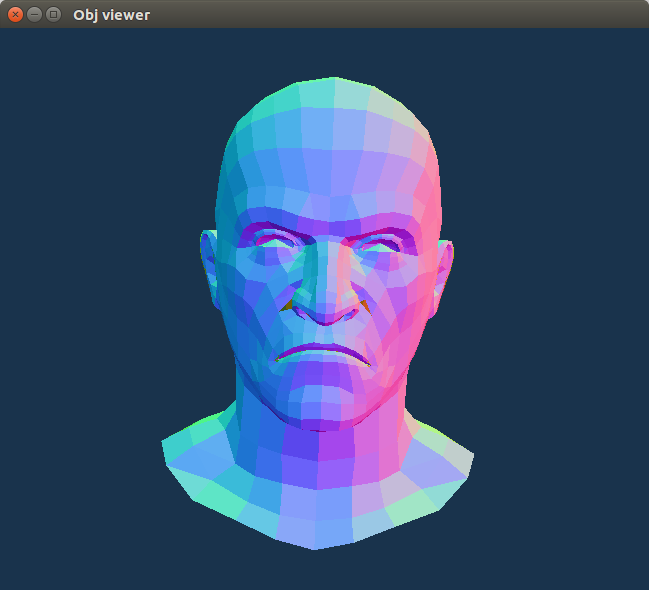
\includegraphics[width=0.4\textwidth]{./figs/rosto-bravo.png}}
  \end{subfigure}
  
  \begin{subfigure}[Pose Nariz Aberto]{\label{fig:pose_nose}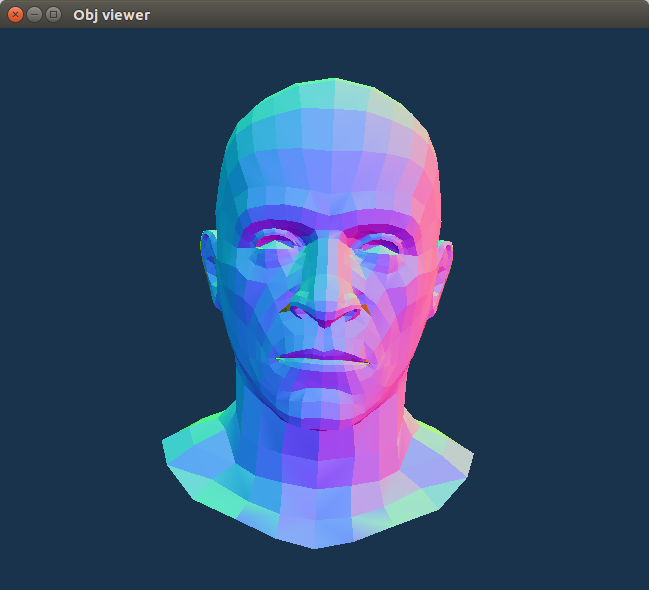
\includegraphics[width=0.4\textwidth]{./figs/nose.png}}
  \end{subfigure}

  \caption{Exemplos de modelos usados como poses pré-definidas.}

  \label{fig:blend-shapes-base-simple-shapes2}
\end{figure}

A Equação \ref{eq:blendshapes} descreve como as poses pré-definidas podem ser
combinadas com a pose neutra de forma a obter  uma quantidade imensa de poses
intermediárias. 

Conectando as etapas apresentas até agora dentro de um laço de execução, os
pesos de mistura são atualizados iterativamente de acordo com o movimento dos
pontos rastreados, produzindo mudanças suaves na forma do modelo resultante
renderizado. A sequência de configurações pelas quais passa o modelo renderizado
a medida que as imagens são capturadas e processadas resultam na animação
computacional que é o objetivo da aplicação.


% O resultado dessa animação pode ser observado na Figura \ref{fig:final_model1}, onde o modelo final é uma pose intermediária entre, essencialmente, o modelo de sorriso e o modelo de boca aberta.

% \begin{figure*}[!htb]
%    \centering
% \begin{tabular}{cc}
%   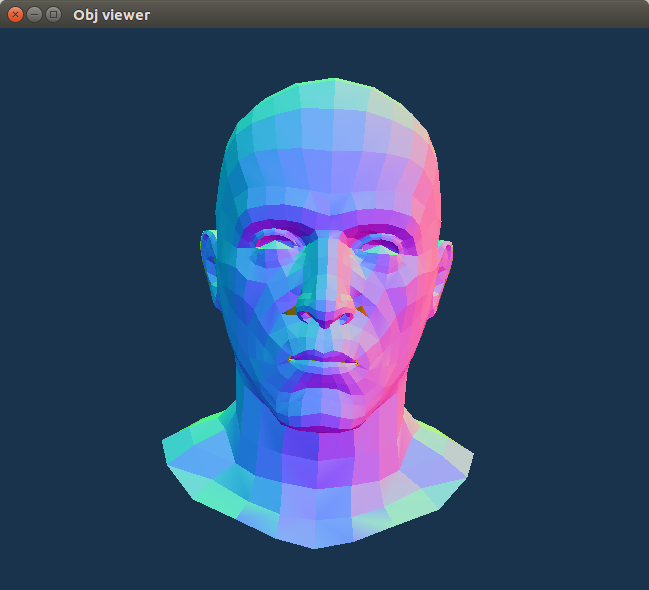
\includegraphics[width=0.4\linewidth]{./figs/mouth-closed.png}
%   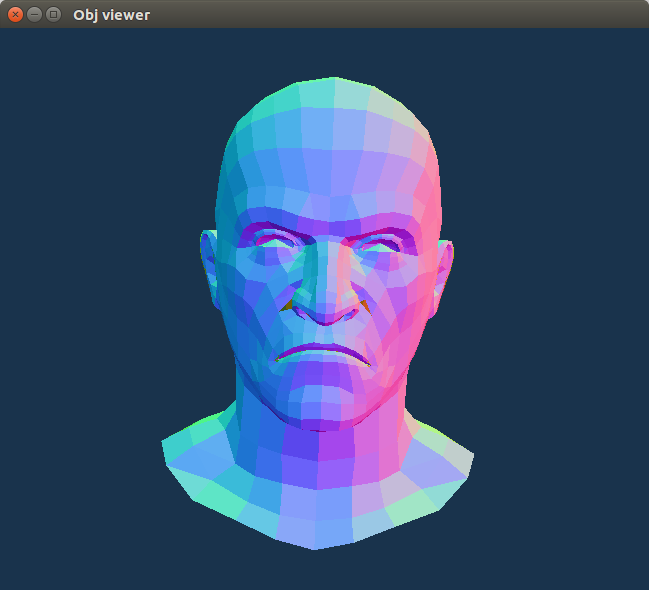
\includegraphics[width=0.4\linewidth]{./figs/rosto-bravo.png}
% \end{tabular}

% \caption{legenda}

% \label{fig:blend-shapes-base-complex-shapes}
% \end{figure*}

% \begin{figure*}[!htb]
%    \centering
% \begin{tabular}{cc}
%   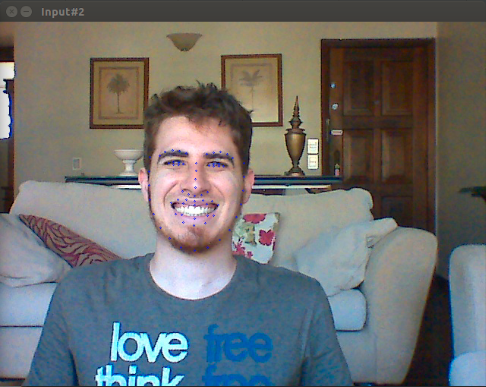
\includegraphics[width=0.4\linewidth]{./figs/TG_pose_inter_input1.png}
%   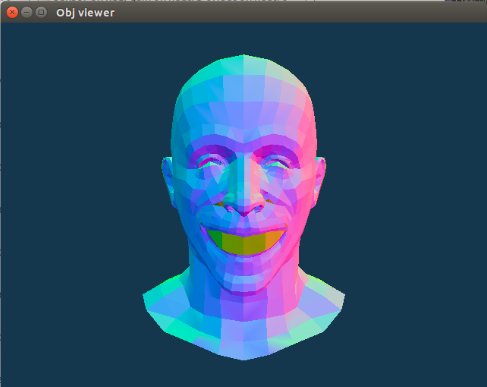
\includegraphics[width=0.4\linewidth]{./figs/TG_pose_inter_model1.png}
% \end{tabular}

% \caption{legenda}

% \label{fig:final_model1}
% \end{figure*}

\section{Experimentos de Validação dos Métodos Utilizados}

Como não se dispõe de um método para medir a qualidade final dos resultados de
modo quantitativo, propõem-se alguns experimentos com o objetivo de validar as
etapas do processo. Os experimentos visam revelar as limitações atuais da
técnica ao medir a precisão de cada etapa.

Uma das dificuldades enfrentadas no experimento é que a aplicação envolve o
rastreamento de um rosto humano e não é encontrada uma boa maneira de substituir
o alvo humano por um objeto que possa ser facilmente fixado e ter a posição
controlada. Com isso, pessoas são utilizadas como parte do experimento e
certamente há erros introduzidos nas medidas. Para exemplificar, em um dos
experimentos propostos o objetivo é tirar várias fotos do usuário há uma
distância fixa, no entanto, é difícil garantir que o alvo não tenha se movido
entre uma foto e outra. Há ainda o problema da iluminação que pode variar
ligeiramente a medida que as horas de experimentos passam. Tendo isso em mente,
o objetivo dos experimentos é que eles forneçam uma ideia das limitações da
técnica e não que sejam uma metodologia precisa de estimação dos erros
envolvidos. 

Tendo em vista que o controle do ambiente e da iluminação não são necessários para o
funcionamento adequado do sistema de animação proposto, não especificamos 
restrições em relação a estes fatores para os experimentos. Também é possível utilizar 
um computador que possua hardware acessível, vale notar que os computadores utilizados 
nos experimentos deste trabalho são \textit{notebooks} com as seguintes especificações: 

Computador 1: Intel® Core™ i7-2630QM CPU @ 2.00GHz × 8; 6GB RAM; GeForce GT 540M/PCIe/SSE2;
Ubuntu 14.04; OpenGL 3.3.

Computador 2: Intel® Core™ i7-4510U CPU @ 2.00GHz × 4; 16GB RAM; Sem placa de vídeo 
dedicada; Ubuntu 16.04; OpenGL 3.3.  

A Figura \ref{fig:exp-montagem} mostra a montagem utilizada nos experimentos que
se seguem. Antes de cada medida, os passos a seguir são tomados como uma
configuração inicial:

\begin{enumerate}

\item O par de câmeras é posicionado na altura do rosto alvo. Seja a direção da
  linha ligando as câmeras chamada de $\vec{A}$.

\item A ponta da trena horizontal é posta no ponto médio entre as câmeras e é
  puxada em direção $\vec{B}$ perpendicular a $\vec{A}$ e no sentido apontando
  para o usuário.

\item O usuário segura a trena e se afasta do par de câmeras se movendo na
  direção $\vec{B}$ até atingir a distância desejada.

\item Nesse ponto uma segunda régua (segmento vermelho na Figura
  \ref{fig:exp-montagem}) é posta verticalmente e ortogonalmente sobre a trena e
  o usuário encosta o nariz na ponta da régua vertical. 

\item Esta é a posição que o ator deve manter durante o resto do experimento o
  mais fielmente possível.

\end{enumerate}

\begin{figure}[!htp]
\centering
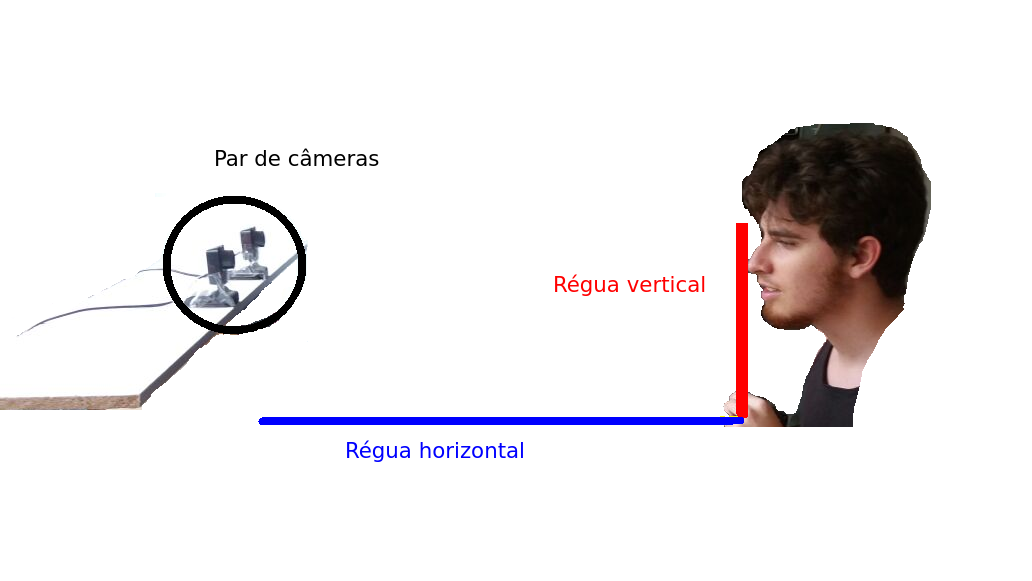
\includegraphics[width=0.8\linewidth]{figs/setupExperimento-comentado-fundo-branco.png}
\caption{\textit{Setup} experimental utilizado para captura repetitiva de fotos do mesmo alvo em várias posições controladas.}
\label{fig:exp-montagem}
\end{figure}

\subsection{Rastreamento de Pontos da Face e Estimação do Tridimensional}

O Rastreamento de Pontos da Face retorna o valor das coordenadas dos pontos em
pixeis, fazendo com que as distâncias entre pares de pontos associados a uma
pose, quando avaliadas diretamente na imagem, mudem à medida que o usuário se
afasta ou se aproxima do sistema de captura. Por outro lado, a técnica de
estimação de profundidade almeja garantir que essas distâncias, agora medidas em
centímetros, se mantenham as mesmas se as distâncias assim se mantiverem no
objeto real. Para mostrar que a recuperação da profundidade está sendo feita de
forma adequada, propõe-se um experimento que irá medir a distância em
centímetros de um par de pontos do rosto, à medida que o usuário se afasta do
par de câmeras. Se o processo for feito como esperado, a distância entre os
pontos do rosto será sempre a mesma, independentemente das distância do alvo às
câmeras.  Outro ponto a ser notado é que para o rastreamento ser considerado
preciso, as distâncias medidas não podem variar no caso de o face alvo estar
imóvel. Para verificar isso, propõe-se também medir o desvio padrão na sequência
de medidas de distância entre dois pontos de uma face imóvel em uma série de
capturas.


Para ambos os experimentos o par de pontos escolhidos para se medir em cada
quadro é composto pelos pontos laterais extremos dos lábios (pontos 48 e 54 na
Figura \ref{fig:tracked-facial-points}). As mesmas imagens capturadas foram
utilizadas em ambos os experimentos.

Para a realização dos experimentos, os seguintes passos foram tomados:

\begin{enumerate}
      
\item A montagem inicial é executada posicionando o nariz do alvo a 40
  centímetros de distância.

\item Capturam-se 30 quadros de cada câmera enquanto o alvo se mantém o mais
  estático possível.

\item Repete-se o processo afastando-se o alvo do par de câmeras 5 centímetros
  em cada etapa, até que se atinja a distância de 80 cm do par de câmeras.

\end{enumerate}

Após a captura, as imagens são entradas aos pares em um programa que:

\begin{enumerate}

\item Aplica o algoritmo de rastreamento dos 66 pontos do rosto no par de
  imagens.

\item Mede a distância entre os pontos 48 e 54 em pixeis para cada câmera.

\item Aplica a técnica de estimação de profundidade para corrigir as coordenadas
  (x,y) de cada ponto detectado

\item Mede a distância entre os pontos 48 e 54 em centímetros.

\end{enumerate}

Para cada par de quadros, os seguintes valores são salvos em arquivo: a
distância entre os pontos 48 e 54 em pixeis da imagem capturada com a câmera 1,
a distância entre os pontos 48 e 54 em pixeis da imagem capturada com a câmera 2
e a distância entre os pontos 48 e 54 estimada em centímetros. 


\subsection{Filtragem Digital}

Neste experimento o objetivo é comparar a sequência de coeficientes de mistura
filtrada e não-filtrada.  Para cada um dos pesos de mistura grava-se um par de
vídeos, um para cada câmera, onde o ator centrado na tela movimenta
intencionalmente os músculos do rosto associados com o peso de mistura que se
quer examinar. 

Apenas um vídeo é gravado para cada pose examinada. Todos os vídeos são gravados
a uma mesma distância da câmera e sobre condição de iluminação semelhante. No
caso de poses simétricas, como o fechar do olho esquerdo e do direito, apenas o
movimento do lado esquerdo do rosto é examinado. Para cada movimento avaliado,
os vídeos gravados são colocados em um programa que aplica o rastreamento visual
dos pontos do rosto e mede apenas a razão de distância considerada (por exemplo,
no vídeo que examina o olho, mede-se somente a abertura dos olhos e no vídeo que
examina o sorrir, apenas o comprimento horizontal dos lábios é medido). 

A razão obtida é entrada independentemente em cada um dos filtros projetados. A
razão medida e a saída de cada um dos filtros é guardada em arquivo para análise
posterior.

O próximo capítulo apresenta os resultados obtidos neste trabalho para cada etapa 
intermediária e para o sistema de animação completo em funcionamento.


